% Methodology section.  Requires \usepackage{tikz} in the preamble.
% All geometry is given in explicit coordinates so no tikz library is needed.

\section{Methodology}
\label{sec:methodology}

We treat the microcode engine as a target architecture rather than as an implementation detail of the x86 interface.
An implementation for it is therefore designed from the operations that the primitive requires and not from an existing x86 instruction sequence.
A design transcribed from native code would inherit decisions that the architectural interface forced and that this interface does not force.

Descending below that interface is worth doing only when a kernel pays an architectural cost that the microcode domain removes and when the removal is larger than the price of the descent.
\Cref{fig:gains} names the four costs we remove and the price we pay for the opportunity.
Each site in that figure corresponds to a family of techniques and a case study is an instance of the same five decisions taken for one primitive.

\begin{figure}[t]
\centering
\footnotesize
\setlength{\fboxsep}{4pt}
\begin{tabular}{@{}c@{\hspace{2.5mm}}c@{}}

\fbox{\begin{minipage}[t][33mm][t]{0.435\linewidth}
\textbf{1.\ Spilled state}\hfill{\scriptsize gain}\\[1pt]
\centering
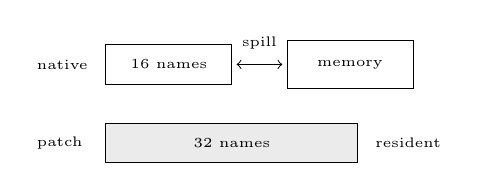
\begin{tikzpicture}[x=1mm,y=1mm,font=\tiny,line width=0.35pt]
  \node[right] at (0,14.5) {native};
  \draw (10,12) rectangle (26,17); \node at (18,14.5) {16 names};
  \draw (33,11.5) rectangle (49,17.5); \node at (41,14.5) {memory};
  \draw[<->] (26.6,14.5) -- (32.4,14.5);
  \node[above] at (29.5,15.2) {spill};
  \node[right] at (0,4.5) {patch};
  \fill[black!8] (10,2) rectangle (42,7);
  \draw (10,2) rectangle (42,7); \node at (26,4.5) {32 names};
  \node[right] at (43,4.5) {resident};
\end{tikzpicture}

{\raggedright\scriptsize residency by traffic accounting $\cdot$ borrowed
register $\cdot$ lifetime reuse across phases\par}
\end{minipage}}
&
\fbox{\begin{minipage}[t][33mm][t]{0.435\linewidth}
\textbf{2.\ Emulated operations}\hfill{\scriptsize gain}\\[1pt]
\centering
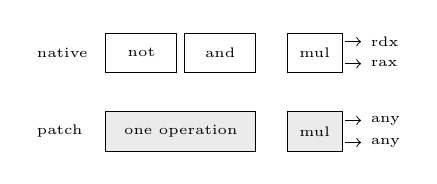
\begin{tikzpicture}[x=1mm,y=1mm,font=\tiny,line width=0.35pt]
  \node[right] at (0,14.5) {native};
  \draw (10,12) rectangle (19,17); \node at (14.5,14.5) {not};
  \draw (20,12) rectangle (29,17); \node at (24.5,14.5) {and};
  \draw (33,12) rectangle (40,17); \node at (36.5,14.5) {mul};
  \draw[->] (40.4,15.9) -- (42.4,15.9); \node[right] at (42.4,15.9) {rdx};
  \draw[->] (40.4,13.1) -- (42.4,13.1); \node[right] at (42.4,13.1) {rax};
  \node[right] at (0,4.5) {patch};
  \fill[black!8] (10,2) rectangle (29,7);
  \draw (10,2) rectangle (29,7); \node at (19.5,4.5) {one operation};
  \fill[black!8] (33,2) rectangle (40,7);
  \draw (33,2) rectangle (40,7); \node at (36.5,4.5) {mul};
  \draw[->] (40.4,5.9) -- (42.4,5.9); \node[right] at (42.4,5.9) {any};
  \draw[->] (40.4,3.1) -- (42.4,3.1); \node[right] at (42.4,3.1) {any};
\end{tikzpicture}

{\raggedright\scriptsize operations absent from the ISA $\cdot$ free
destinations $\cdot$ selection on measured cost\par}
\end{minipage}}
\\[2.5mm]

\fbox{\begin{minipage}[t][33mm][t]{0.435\linewidth}
\textbf{3.\ Serialised carries}\hfill{\scriptsize gain}\\[1pt]
\centering
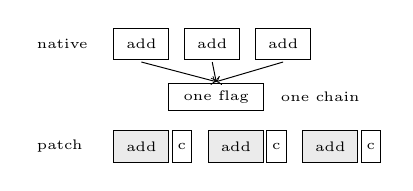
\begin{tikzpicture}[x=1mm,y=1mm,font=\tiny,line width=0.35pt]
  \node[right] at (0,17) {native};
  \foreach \x in {11,20,29}{
    \draw (\x,15) rectangle (\x+7,19); \node at (\x+3.5,17) {add};
    \draw[->] (\x+3.5,14.7) -- (24,12.2);}
  \draw (18,8.5) rectangle (30,12); \node at (24,10.25) {one flag};
  \node[right] at (31,10.25) {one chain};
  \node[right] at (0,4) {patch};
  \foreach \x in {11,23,35}{
    \fill[black!8] (\x,2) rectangle (\x+7,6);
    \draw (\x,2) rectangle (\x+7,6); \node at (\x+3.5,4) {add};
    \draw (\x+7.4,2) rectangle (\x+9.9,6); \node at (\x+8.65,4) {c};}
\end{tikzpicture}

{\raggedright\scriptsize independent condition state $\cdot$ matched
representation $\cdot$ parallel restructuring\par}
\end{minipage}}
&
\fbox{\begin{minipage}[t][33mm][t]{0.435\linewidth}
\textbf{4.\ Dispatch and supply}\hfill{\scriptsize gain}\\[1pt]
\centering
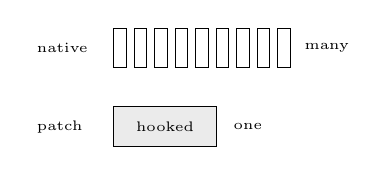
\begin{tikzpicture}[x=1mm,y=1mm,font=\tiny,line width=0.35pt]
  \node[right] at (0,14.5) {native};
  \foreach \x in {11,13.6,16.2,18.8,21.4,24,26.6,29.2,31.8}{
    \draw (\x,12) rectangle (\x+1.6,17);}
  \node[right] at (34,14.5) {many};
  \node[right] at (0,4.5) {patch};
  \fill[black!8] (11,2) rectangle (24,7);
  \draw (11,2) rectangle (24,7); \node at (17.5,4.5) {hooked};
  \node[right] at (25,4.5) {one};
\end{tikzpicture}

{\raggedright\scriptsize one host instruction $\cdot$ fixed register interface
$\cdot$ chaining between firings $\cdot$ wrapper order\par}
\end{minipage}}
\\[2.5mm]

\multicolumn{2}{@{}c@{}}{%
\fbox{\begin{minipage}[t][33mm][t]{0.925\linewidth}
\textbf{5.\ The price of the descent}\hfill{\scriptsize cost}\\[1pt]
\centering
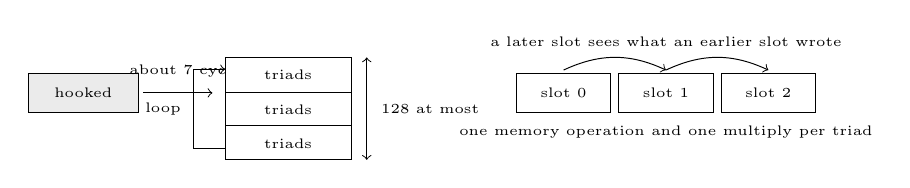
\begin{tikzpicture}[x=1mm,y=1mm,font=\tiny,line width=0.35pt]
  \fill[black!8] (2,10) rectangle (16,15);
  \draw (2,10) rectangle (16,15); \node at (9,12.5) {hooked};
  \draw[->] (16.6,12.5) -- (25.4,12.5);
  \node[above] at (21,13.2) {about 7 cyc};
  \draw (27,4) rectangle (43,17);
  \draw (27,8.3) -- (43,8.3);
  \draw (27,12.6) -- (43,12.6);
  \node at (35,14.8) {triads}; \node at (35,10.4) {triads}; \node at (35,6.1) {triads};
  \draw[->] (27,5.5) -- (23,5.5) -- (23,15.5) -- (27,15.5);
  \node[left] at (22.6,10.5) {loop};
  \draw[<->] (45,4) -- (45,17);
  \node[right] at (45.6,10.5) {128 at most};
  \foreach \i in {0,1,2}{\draw (64+\i*13,10) rectangle (76+\i*13,15);}
  \node at (70,12.5) {slot 0}; \node at (83,12.5) {slot 1}; \node at (96,12.5) {slot 2};
  \draw[->] (70,15.4) to[bend left=25] (83,15.4);
  \draw[->] (83,15.4) to[bend left=25] (96,15.4);
  \node at (83,19) {a later slot sees what an earlier slot wrote};
  \node at (83,7.5) {one memory operation and one multiply per triad};
\end{tikzpicture}

{\raggedright\scriptsize maximum granularity $\cdot$ microsequencer loop
$\cdot$ several hooks $\cdot$ work partition $\cdot$ specialised kernels
$\cdot$ slot packing $\cdot$ boundary merging\par}
\end{minipage}}}

\end{tabular}
\caption{The four architectural costs a microcode implementation removes and the price it pays for doing so.
Panels~1 to~4 contrast a native implementation with a patch at each site.
The register file doubles and the working set stops moving through memory.
An instruction pair collapses into one operation and a multiply writes where the patch chooses rather than where the architecture pins it.
Condition state held with a destination register replaces the single architectural flag that admits one carry chain.
A long instruction sequence becomes one macroinstruction.
Panel~5 shows what this costs.
Entry is priced and capacity is bounded and the schedule is static.
Each panel lists the family of techniques that applies at its site.}
\label{fig:gains}
\end{figure}

\paragraph{Spilled state.}
The architectural register file is smaller than the working set of a cryptographic kernel so native code moves part of that set through memory.
A patch reaches sixteen further registers that no architectural instruction can name which brings the file to 32 names.
We hold the whole working set of one firing in those names so that the kernel spills nothing while it executes.
Three techniques make that budget hold.
We decide what stays resident by counting the reads a value receives inside one firing rather than across the primitive.
We borrow an architectural register whose role is irrelevant while the patch runs and restore it before the patch returns.
We reuse a register that is dead at a phase boundary as scratch for the next phase which needs an allocation planned across the whole kernel.

\paragraph{Emulated operations.}
An operation the instruction set does not provide must be assembled from the operations it does provide.
The engine exposes operations that this core does not expose to software and one of them can replace a pair of instructions that native code is forced into.
It also leaves the destination of an operation to the patch where the architectural form pins it to a fixed register.
That freedom removes the copies which surround such an instruction and it lets a staged operand become the initial value of an accumulator.
Selection is made on measured cost because some micro operations look ordinary and trap to a slow path.
The same arithmetic step is sometimes implemented in two ways inside one patch according to whether it lies on the critical path.

\paragraph{Serialised carries.}
Architectural arithmetic records its carry in one flags register so an instruction sequence can hold one carry chain at a time.
The engine instead leaves condition state with the destination register of an arithmetic operation and a patch can keep several chains live at once.
We select the representation whose dependency structure the engine can hold rather than the one native code prefers.
We then replace a serial accumulation with independent accumulations wherever the engine is limited by issue capacity rather than by latency.
A representation that funnels every overflow through a single carry forfeits the technique and we measure such a representation as a control.

\paragraph{Dispatch and instruction supply.}
A native kernel is a long instruction sequence that the front end must fetch and decode and retire.
The same kernel behind a hooked macroinstruction occupies one architectural instruction so those resources carry only the operand transfer.
The hooked instruction has no calling convention so we choose which architectural registers carry the inputs and the outputs of a kernel.
The host can then precompute values into those registers and consecutive firings can hand values over in registers instead of through memory.
The native instructions that surround the hooked instruction belong to the kernel and are ordered with it because their memory order can dominate everything the patch does.

\paragraph{The price of the descent.}
Redirection into patch RAM costs about seven cycles and a complete invocation about sixteen once operand marshalling is counted.
\Cref{fig:decodeandpatch} shows the mechanism that performs the redirection.
Patch RAM holds 128 triads and no temporary register survives a firing.
Each triad issues three micro operations and an independent operation costs about a third of a cycle against about 1.33 for a multiply.
Five techniques pay this price.
We place the largest unit of the computation that fits in patch RAM behind each redirection.
We keep control flow inside the microsequencer so that a loop runs a computation larger than the patch itself in one firing without losing its resident state.
We redirect more than one macroinstruction so that a specialised kernel coexists with the general one and earns its capacity where it performs less work.
We leave in native code the work that is cheaper there than the capacity it would consume.
We pack operations into every slot and let consecutive phases share the triad at their boundary and we use the sequential semantics of the slots to hold a dependent chain inside one triad.

\subsection{The order of the decisions}
\label{sec:method-order}

The five families are applied in a fixed order because each decision constrains the next.
We place the boundary first and fix how much of the dominant computation runs behind one firing.
That decision is structural rather than an optimisation because a computation divided across two firings pays the entry price twice.
We then choose the representation and then plan residency and then select operations and then schedule them into triads.
Validation and measurement come last and return their result to the first decision rather than to the last.

\subsection{Development and validation}
\label{sec:method-dev}

An incorrect patch is not reported as an exception and returns a wrong value or hangs the core or halts the machine.
One unverified operation encoding halted ours.
We therefore write no kernel as triads.
Each kernel is a program that emits an intermediate form of micro operations and a simulator executes that form against an independent reference before anything is installed.
A separate audit checks the hardware rules the simulator cannot observe such as a register read before it is written and a packer then lowers the validated form into triads.
Every kernel is validated again on the hardware that will time it against published known answer constants.

We rank candidate designs with a cost model and accept none on its prediction.
Two schedules of one kernel with an identical operation count and triad count and dependency depth measured 5.7 cycles apart so every candidate returns to hardware.
All results come from one core pinned to its base frequency with turbo disabled and every contender is timed by one process through one harness across 24 compiler and optimisation configurations.
We measure the kernel alone and then inside a fixed surrounding implementation and then as a complete implementation.
We attribute the outcome with ablations that remove one technique and leave the rest of the implementation unchanged.

\begin{figure}[tbp]
  \centering
  \includegraphics[width=0.9\linewidth]{DecoderAndPatch.png}
  \caption{Decode path on Goldmont and the effect of a microcode patch.
  Macroinstructions decoded by the microsequencer have their MSROM address checked against the match registers.
  An unmatched address (\code{rdrand}) is served from the microcode ROM while a matched address (\code{cpuid} redirected to \uaddr{74dc}) is served from the microcode RAM so that our custom triads are emitted in place of the original ones.}
  \label{fig:decodeandpatch}
\end{figure}
